

\dev{Marin Malory}{\cite{Cormen}}

\textit{Ce développement a pour but de présenter une structure de donnée arborescente implémentant un dictionnaire tout en prenant en compte la hiérarchie mémoire. Il trouve alors tout naturellement sa place dans les leçons \ref{L4}, \ref{L6}, \ref{L10} et \ref{L15}. Si la leçon \ref{L16} parle de hiérarchie mémoire, ce développement peut s'y intégrer. 
Enfin, avec un point de vue base de données, les B-arbres peuvent servir en indexation afin d'optimiser certaines requêtes. En modifiant la mise en contexte, ce développement s'intègre alors dans les leçons \ref{L18}, \ref{L22} et \ref{L23}.}

\paragraph{Motivation et exemple.}
Dans le cas d’une grande quantité d’information, il est parfois nécessaire d’utiliser des supports de stockage dont le temps de réponse pour une lecture est élevé (disque dur, ...). Pour implanter une structure de dictionnaire dans ce cas, on préférera contracter notre ABR afin de faire moins d'appels à la mémoire lente.

\begin{example}[Un B-arbre d'ordre $2$ et de hauteur $2$]~

\begin{center}
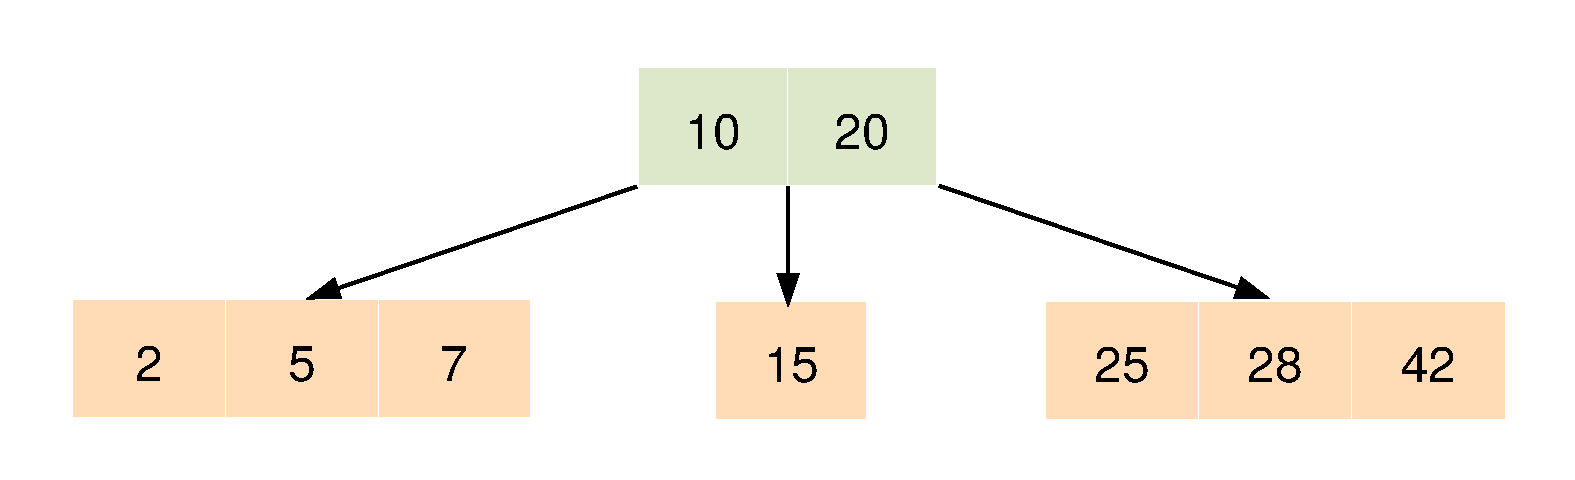
\includegraphics[scale=0.5]{Developpements/B-arbres/exemple.pdf}
\end{center}
\end{example}

\paragraph{Définition.}

\begin{definition}[B-arbre]

Soit un entier $t\geq 2$. On appelle B-arbre d'ordre $t$ un arbre vérifiant les invariants suivants :
\begin{itemize}
\item Chaque nœud $x$ contient les attribut suivants :
\begin{enumerate}
\item le booléen $x.\text{feuille}$ (VRAI si $X$ est une feuille, FAUX sinon) ;
\item le nombre $x.n$ de clés dans ce nœud  ;
\item le tableau trié $x.\text{clé}$ de taille $x.n$ contenant les clés de ce noeud (numéroté de $1$ à $x.n$) ;
\item le tableau $x.\text{fils}$ de taille $x.n +1$ contenant l'ensemble des enfants du nœud $x$ (numéroté de $0$ à $x.n$).
\end{enumerate}
\item pour tout nœud $x$, toute clé $k_i$ apparaissant dans le fils $x.\text{fils}_i$, on a $k_{i-1} \leq x.\text{clé}_i \leq k_i$ ($1\leq i \leq n$).
\item toutes les feuilles ont la même profondeur $h$;
\item pour tout noeud $x$ non racine, on a $t-1 \leq x.n \leq 2t-1$ ;
\item la racine $x_0$ vérifie $1\leq x_0.n \leq 2t-1$.
\end{itemize}
\end{definition}~\newline

Ici, au vu de son utilisation, on suppose le B-arbre stocké dans une mémoire auxiliaire d'accès lent, on va donc compter notre complexité en fonction du nombre de lecture et d'écriture dans cette mémoire. On considère deux fonctions $\mathbf{LIRE}$ et $\mathbf{ECRIRE}$ permettant d'accéder à notre mémoire auxiliaire.



\paragraph{Recherche dans un tel arbre.}
La fonction de recherche dans un B-arbres ressemble beaucoup à la recherche dans un ABR, sauf que dans chaque nœud, il faut chercher le bon intervalle, et que la complexité sera évaluée en fonction d'appel à la fonction $\mathbf{LIRE}$. On suppose que notre racine est en mémoire principale, il n'y a donc pas besoin de faire de appel à $\mathbf{LIRE}$. 

\begin{algorithm}
\Donnees{un noeud $x$ et une clé $c$}
\Res{si $c$ est dans un nœud $y$ de l'arbre, on renvoie $y$ et sa place dans le nœud, sinon on renvoie NIL.}
\caption{Recherche($x$,$c$)}

\# Recherche du bon intervalle ; \\
trouve, $i \leftarrow$ Dichotomie($x.\text{clé}$, $c$) ;\\
\Si{trouve}{
	\Retour{$x$, $i$}
}
\Si{$x.\text{feuille}$}{
	\Retour{NIL}
}
$ f \leftarrow \mathbf{LIRE}(x.\text{fils}_{i-1})$;\\
\Retour{Recherche($f$, $c$)}
\end{algorithm}

On va maintenant étudier la complexité de notre algorithme et comparer à la complexité si on avait utiliser un ABR, c'est-à-dire un B-arbre d'ordre $2$.

\begin{theorem}
Dans un B-arbre $T$ d'ordre $t\geq 2$ contenant $n$ clés, sa hauteur $h$ vérifie 
$$
h \leq \ln_t \left( \frac{n+1}{2}\right)
$$
\end{theorem}

\begin{proof}
Par définition, $T$ contient au moins une clé à la racine, et donc sa racine possède au moins $2$ enfants. On a donc :
\begin{itemize}
\item au moins $1$ nœud à la profondeur $0$ ;
\item au moins $2$ nœuds à la profondeur $1$ ;
\item au moins $2t$ nœuds à la profondeur $2$...
\end{itemize}
On montre alors par récurrence immédiate qu'on a au moins $2t^{i-1}$ nœuds à la profondeur $i$. Puisque chaque nœud contient au moins $(t-1)$ clés, on a :
$$
n \geq 1+(t-1) \sum_{i=1}^h 2t^{i-1} = 1 +2(t-1) \left( \frac{t^h -1}{t-1} \right) = 2t^h -1
$$
Le résultat en découle alors directement.
\end{proof}

Étant donné un B-arbre $T$ de racine $x_0$, la fonction Recherche(x,c) fait $h$ appels à $\mathbf{LIRE}$ dans le pire des cas, que l'on peut borner via le théorème ci-dessus.


\paragraph{Insertion dans un B-arbre.} Ici les choses se compliquent puisque l'insertion est moins évidente. Il y a des situations qui peuvent poser problème, par exemple si l'arbre est déjà plein.\newline

\textbf{Idée de l'algorithme :} sur l'entrée $c$ et le nœud $x$,
\begin{itemize}
\item On va à la feuille correspondante en choisissant les chemins via les intervalles ;
\item Si la feuille possède strictement moins de $2t-1$ étiquettes, on peut insérer $c$ ;
\item Sinon, en notant $c_1,...,c_{2t}$ les nouvelles étiquettes de cette feuilles (avec $c=c_{2t}$), on sépare cette feuilles en deux feuilles d'étiquettes $c_1,...,c_{t-1}$ et $c_{t+1},...,c_{2t}$, et on remonte $c_t$ comme séparateur dans le parent ;
\item Si le parent contient alors trop d'étiquettes, on le coupe en deux de la même manière et ainsi de suite jusqu'à la racine.
\item Si la racine doit être coupée en deux, on crée une nouvelle racine qui ne contiendra qu'une étiquette.
\end{itemize}
